% Full system architecture of the Comorbidity-Aware Meta-Bayesian framework.
% Standalone figure: pdflatex architecture_full.tex  ->  architecture_full.pdf
% It is included, at full width, in the deck (slide 6) and in the report (Figure 4.1).
%
% Status colours:  solid green  = complete and verified (Modules 1-3)
%                  dashed blue  = design only; nothing is trained and no result exists (Modules 4-6)
% Counts and shapes are those of the implemented pipeline; Modules 4-6 follow the
% Review I design (report Sections 4.4 and 4.5).
\documentclass[tikz,border=1.5pt]{standalone}
\usepackage[T1]{fontenc}
\usepackage{lmodern}
\usepackage{amsmath,amssymb}
\renewcommand{\familydefault}{\sfdefault}
\usetikzlibrary{arrows.meta,calc}
\hyphenpenalty=10000 \exhyphenpenalty=10000 \tolerance=9999 \emergencystretch=3em

\definecolor{UBlue}{RGB}{16,62,110}
\definecolor{LBlue}{RGB}{232,242,252}
\definecolor{DGreen}{RGB}{27,122,61}
\definecolor{LGreen}{RGB}{228,243,233}
\definecolor{ClinFill}{RGB}{255,243,205}
\definecolor{ClinLine}{RGB}{176,110,0}
\definecolor{Ink}{RGB}{38,46,58}

% one bullet line with a hanging indent; \outl is the module's output line
\newcommand{\bl}[1]{\hangindent=0.25cm \hangafter=1 \makebox[0.25cm][l]{$\scriptstyle\bullet$}#1\par}
\newcommand{\outl}[1]{\par\vspace{1.5pt}\hangindent=0.4cm \hangafter=1 \makebox[0.4cm][l]{\textbf{$\rightarrow$}}#1\par}

\begin{document}
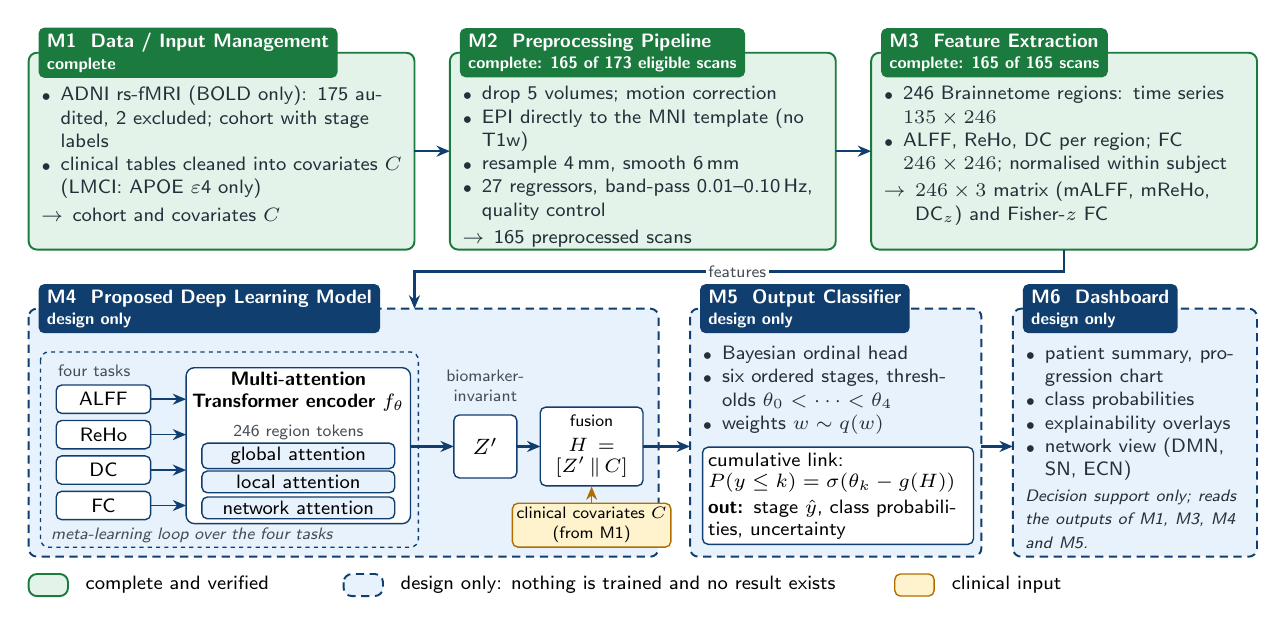
\begin{tikzpicture}[x=1cm,y=1cm,
    font=\fontsize{7}{8.4}\selectfont\color{Ink},
    >={Stealth[length=1.7mm,width=1.4mm]},
    done/.style={draw=DGreen,fill=LGreen,line width=0.7pt,rounded corners=3pt},
    plan/.style={draw=UBlue,fill=LBlue,line width=0.7pt,rounded corners=3pt,dash pattern=on 3pt off 2pt},
    tab/.style={rounded corners=2pt,text=white,inner xsep=3pt,inner ysep=2pt,anchor=west,align=left,
                font=\bfseries\fontsize{7.2}{8.2}\selectfont},
    chip/.style={draw=UBlue,fill=white,rounded corners=2pt,line width=0.5pt,align=center,
                 inner sep=1.5pt,font=\fontsize{6.8}{7.8}\selectfont},
    flow/.style={->,line width=0.9pt,draw=UBlue},
    small/.style={font=\fontsize{6}{7}\selectfont,text=Ink!85}]

% ------------------------------------------------------------------ row 1 (built)
\draw[done] (0,0) rectangle (4.9,-2.5);
\draw[done] (5.35,0) rectangle (10.25,-2.5);
\draw[done] (10.7,0) rectangle (15.6,-2.5);

\node[tab,fill=DGreen] at (0.12,0) {M1\ \ Data / Input Management\\[-0.5pt]{\itshape\fontsize{6}{7}\selectfont complete}};
\node[tab,fill=DGreen] at (5.47,0) {M2\ \ Preprocessing Pipeline\\[-0.5pt]{\itshape\fontsize{6}{7}\selectfont complete: 165 of 173 eligible scans}};
\node[tab,fill=DGreen] at (10.82,0) {M3\ \ Feature Extraction\\[-0.5pt]{\itshape\fontsize{6}{7}\selectfont complete: 165 of 165 scans}};

\node[anchor=north west,text width=4.6cm,align=left,inner sep=0pt] at (0.15,-0.42) {%
  \bl{ADNI rs-fMRI (BOLD only): 175 audited, 2 excluded; cohort with stage labels}
  \bl{clinical tables cleaned into covariates $C$ (LMCI: APOE $\varepsilon$4 only)}
  \outl{cohort and covariates $C$}};
\node[anchor=north west,text width=4.6cm,align=left,inner sep=0pt] at (5.5,-0.42) {%
  \bl{drop 5 volumes; motion correction}
  \bl{EPI directly to the MNI template (no T1w)}
  \bl{resample 4\,mm, smooth 6\,mm}
  \bl{27 regressors, band-pass \mbox{0.01--0.10\,Hz}, quality control}
  \outl{165 preprocessed scans}};
\node[anchor=north west,text width=4.6cm,align=left,inner sep=0pt] at (10.85,-0.42) {%
  \bl{246 Brainnetome regions: time series $135\times246$}
  \bl{ALFF, ReHo, DC per region; FC \mbox{$246\times246$}; normalised within subject}
  \outl{\mbox{$246\times3$} matrix (mALFF, mReHo, DC$_z$) and Fisher-$z$ FC}};

\draw[flow] (4.9,-1.25) -- (5.35,-1.25);
\draw[flow] (10.25,-1.25) -- (10.7,-1.25);

% ------------------------------------------------------------------ row 2 (design)
\draw[plan] (0,-3.25) rectangle (8.0,-6.4);
\draw[plan] (8.4,-3.25) rectangle (12.1,-6.4);
\draw[plan] (12.5,-3.25) rectangle (15.6,-6.4);

\node[tab,fill=UBlue] at (0.12,-3.25) {M4\ \ Proposed Deep Learning Model\\[-0.5pt]{\itshape\fontsize{6}{7}\selectfont design only}};
\node[tab,fill=UBlue] at (8.52,-3.25) {M5\ \ Output Classifier\\[-0.5pt]{\itshape\fontsize{6}{7}\selectfont design only}};
\node[tab,fill=UBlue] at (12.62,-3.25) {M6\ \ Dashboard\\[-0.5pt]{\itshape\fontsize{6}{7}\selectfont design only}};

% wrap arrow: features leave M3 and enter M4
\draw[flow] (13.15,-2.5) -- (13.15,-2.78) -- (4.9,-2.78) -- (4.9,-3.25);
\node[fill=white,inner sep=1pt,small] at (9.0,-2.78) {features};

% ---- M4: meta-learning group, encoder, fusion
\draw[UBlue,line width=0.5pt,dash pattern=on 1.5pt off 1.5pt,rounded corners=3pt] (0.15,-3.8) rectangle (4.95,-6.28);
\node[small,anchor=north west] at (0.25,-3.84) {four tasks};
\foreach \t/\y in {ALFF/-4.4,ReHo/-4.85,DC/-5.3,FC/-5.75}{
  \node[chip,minimum width=1.2cm,minimum height=0.36cm] at (0.95,\y) {\t};
  \draw[->,line width=0.6pt,draw=UBlue] (1.55,\y) -- (2.0,\y);
}
\draw[chip,rounded corners=3pt] (2.0,-4.0) rectangle (4.85,-5.98);
\node[anchor=north,text width=2.7cm,align=center,inner sep=0pt,font=\bfseries\fontsize{6.8}{7.8}\selectfont]
  at (3.425,-4.05) {Multi-attention Transformer encoder $f_\theta$};
\node[small,anchor=north] at (3.425,-4.6) {246 region tokens};
\foreach \a/\y in {global attention/-5.12,local attention/-5.45,network attention/-5.78}{
  \node[chip,fill=LBlue,minimum width=2.45cm,minimum height=0.27cm] at (3.425,\y) {\a};
}
\node[small,anchor=north west,text width=4.6cm,inner sep=0pt] at (0.28,-6.03) {\itshape meta-learning loop over the four tasks};

\draw[flow] (4.85,-5.0) -- (5.4,-5.0);
\node[chip,minimum width=0.8cm,minimum height=0.8cm,font=\bfseries\fontsize{8}{9}\selectfont] (zp) at (5.8,-5.0) {$Z'$};
\node[small,anchor=south,align=center] at (5.8,-4.55) {biomarker-\\invariant};
\draw[flow] (6.2,-5.0) -- (6.5,-5.0);
\node[chip,minimum width=1.3cm,minimum height=1.0cm,text width=1.2cm] (fus) at (7.15,-5.0)
  {\fontsize{6}{7}\selectfont fusion\\[1pt]\fontsize{7}{8}\selectfont $H=[Z'\,\|\,C]$};
\node[draw=ClinLine,fill=ClinFill,rounded corners=2pt,line width=0.5pt,align=center,inner sep=1.5pt,
      font=\fontsize{6.2}{7.2}\selectfont,minimum width=1.3cm,minimum height=0.55cm] (cc) at (7.15,-6.0)
  {clinical covariates $C$\\ (from M1)};
\draw[->,line width=0.6pt,draw=ClinLine] (cc.north) -- (fus.south);
\draw[flow] (7.8,-5.0) -- (8.4,-5.0);

% ---- M5
\node[anchor=north west,text width=3.4cm,align=left,inner sep=0pt] at (8.55,-3.72) {%
  \bl{Bayesian ordinal head}
  \bl{six ordered stages, thresholds $\theta_0<\dots<\theta_4$}
  \bl{weights $w\sim q(w)$}};
\node[draw=UBlue,fill=white,rounded corners=2pt,line width=0.5pt,anchor=north west,text width=3.3cm,align=left,
      inner sep=2pt,font=\fontsize{6.6}{7.8}\selectfont] at (8.55,-5.0) {%
  cumulative link:\\ $P(y\le k)=\sigma(\theta_k-g(H))$\\[1.5pt]
  \textbf{out:} stage $\hat y$, class probabilities, uncertainty};
\draw[flow] (12.1,-5.0) -- (12.5,-5.0);

% ---- M6
\node[anchor=north west,text width=2.85cm,align=left,inner sep=0pt] at (12.65,-3.72) {%
  \bl{patient summary, progression chart}
  \bl{class probabilities}
  \bl{explainability overlays}
  \bl{network view (DMN, SN, ECN)}
  \par\vspace{1pt}{\fontsize{6.2}{7.2}\selectfont\itshape Decision support only; reads the outputs of M1, M3, M4 and M5.}};

% ------------------------------------------------------------------ legend
\draw[done] (0,-6.62) rectangle (0.5,-6.9);
\node[anchor=west,font=\fontsize{6.6}{7.6}\selectfont] at (0.6,-6.76) {complete and verified};
\draw[plan] (4.0,-6.62) rectangle (4.5,-6.9);
\node[anchor=west,font=\fontsize{6.6}{7.6}\selectfont] at (4.6,-6.76) {design only: nothing is trained and no result exists};
\draw[draw=ClinLine,fill=ClinFill,rounded corners=2pt,line width=0.5pt] (11.0,-6.62) rectangle (11.5,-6.9);
\node[anchor=west,font=\fontsize{6.6}{7.6}\selectfont] at (11.6,-6.76) {clinical input};
\end{tikzpicture}
\end{document}
